\documentclass{article}

% Paquetes necesarios
\usepackage[utf8]{inputenc} % Codificación de entrada UTF-8
\usepackage[spanish]{babel} % Idioma español
\usepackage{graphicx} % Para incluir imágenes
\usepackage{lipsum} % Generador de texto de relleno
\usepackage{multicol} % Para dividir el texto en columnas

% Título y autor del artículo
\title{Guía rápida de LaTex}
\author{Alexi Mendoza\\ \and Mary Vera \\ }
\date{\today} % O puedes especificar una fecha específica

\begin{document}

\maketitle % Generar el título

\begin{abstract}
Overleaf es una herramienta de publicación y redacción colaborativa en línea que hace que todo el proceso de redacción, edición y publicación de documentos científicos sea mucho más rápido y sencillo. Overleaf pone a tu disposición un editor LaTeX fácil de usar que incluye colaboración en tiempo real y compilación automática, de modo que se visualiza el resultado a medida que se escribe.
\end{abstract}

\section{Introducción}
LaTeX es un sistema de preparación de documentos. Con él puedes preparar manuscritos, artículos de revista, cartas, tesis, presentaciones y cualquier tipo de documento que quisieras imprimir en papel o mostrar en pantalla.

\begin{figure*}[ht]
    \centering
    \begin{minipage}[b]{0.45\linewidth}
        \centering
        
\includegraphics[width=\linewidth]{latex.png} % Cambia "imagen1.jpg" por el nombre de tu primera imagen
        \caption{Overleaf}
        \label{fig:imagen1}
    \end{minipage}
    \hspace{0.5cm}
    \begin{minipage}[b]{0.45\linewidth}
        \centering
        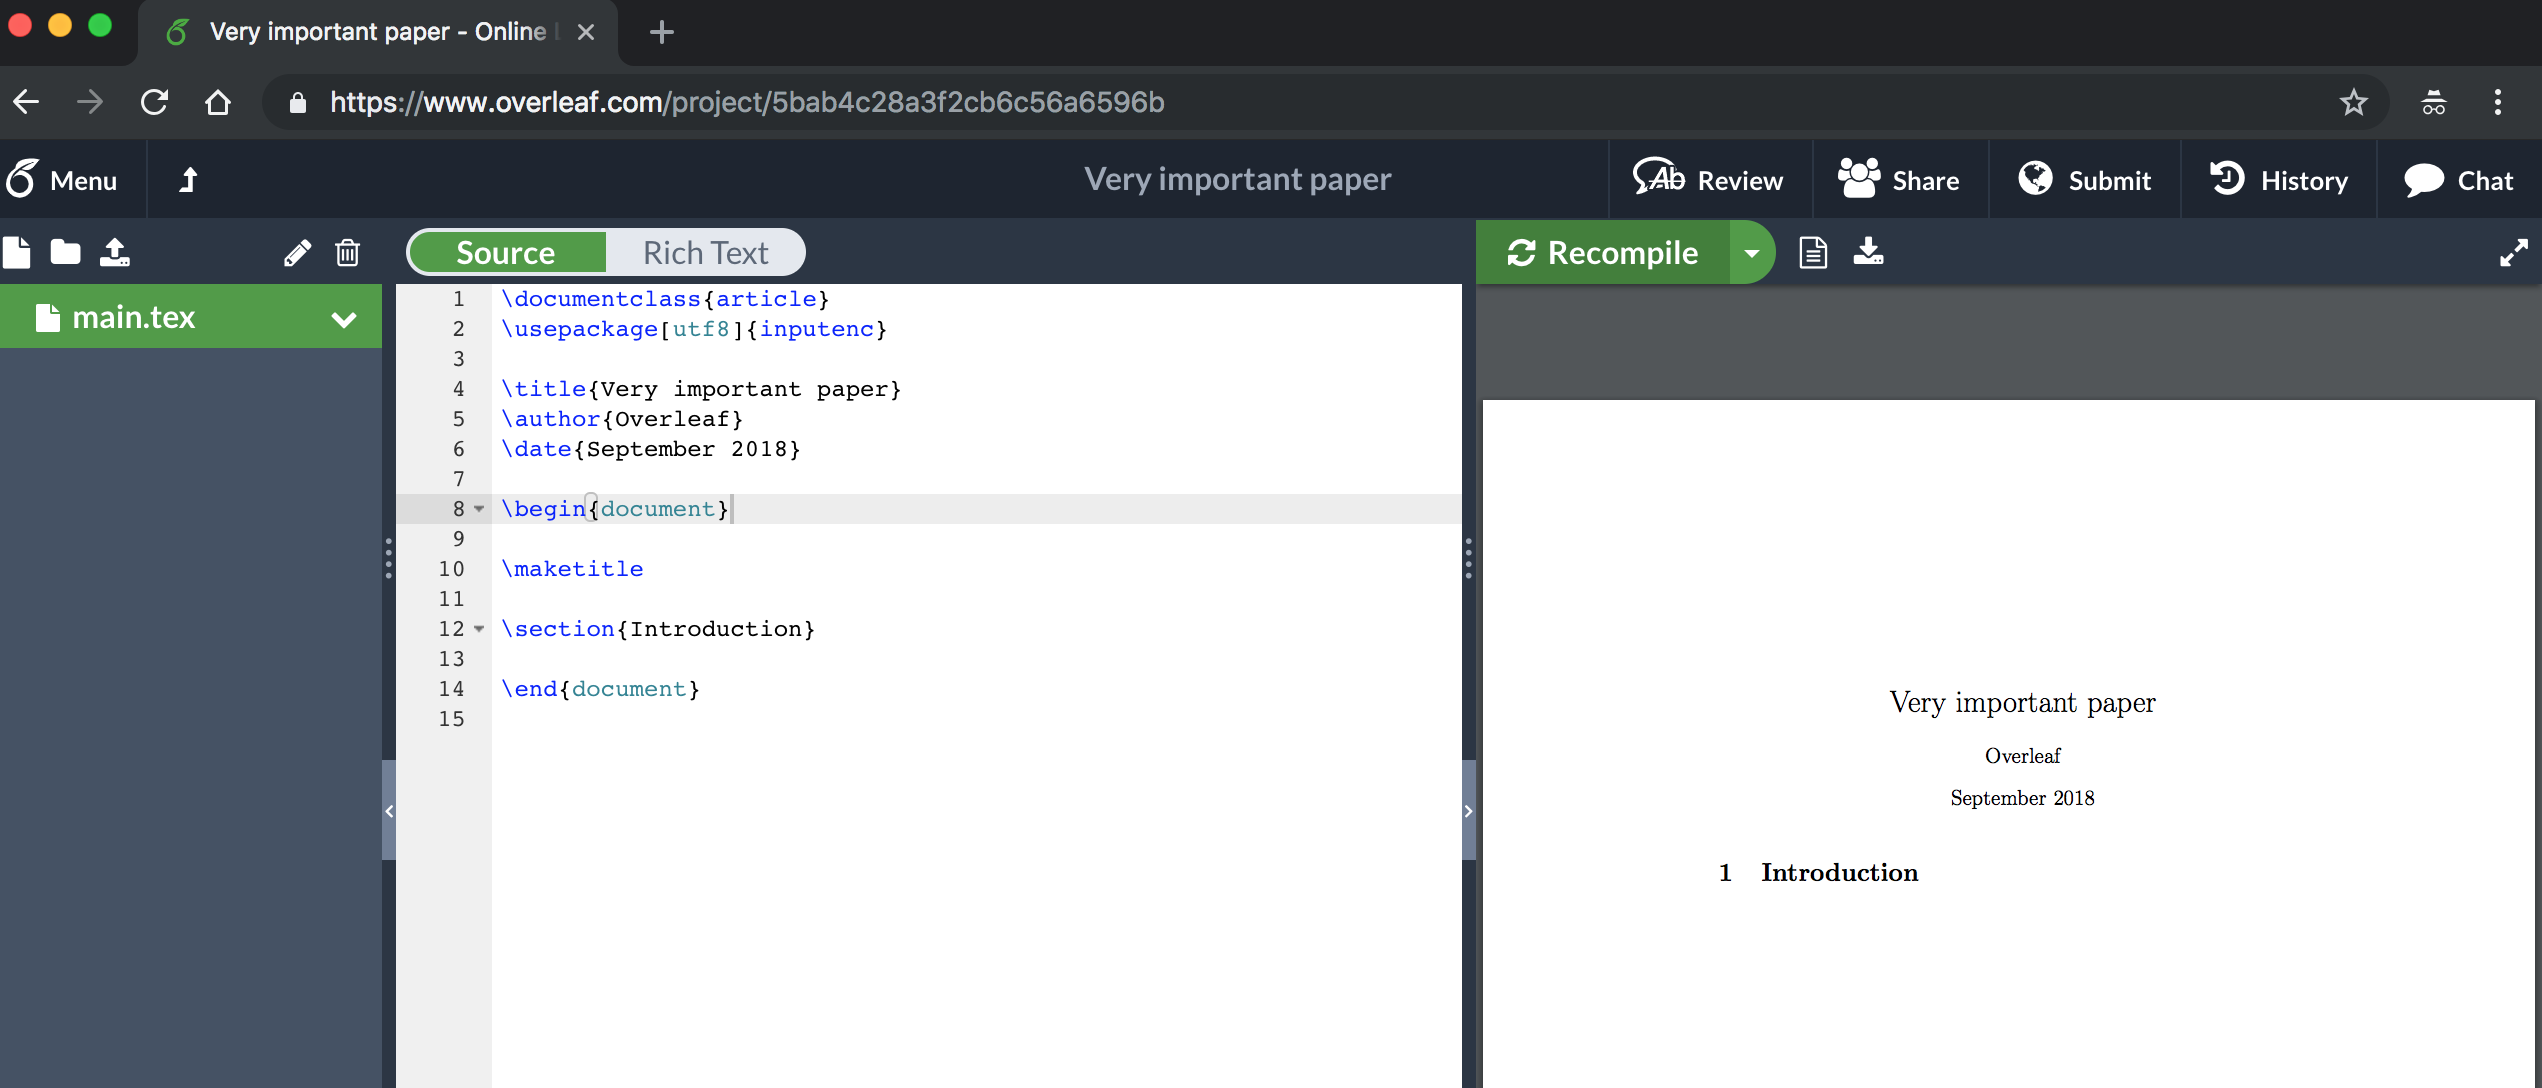
\includegraphics[width=\linewidth]{latex1.png} % Cambia "imagen2.jpg" por el nombre de tu segunda imagen
        \caption{En la web}
        \label{fig:imagen2}
    \end{minipage}
\end{figure*}

\begin{multicols}{2} % Inicio de la división en dos columnas
\section{¿Por qué debería de usar LaTeX?}
Existiendo otras alternativas más convencionales para producir documentos, como Word de Microsoft, es natural preguntarse porque debería uno tomarse la molestia de aprender a usar LaTeX.

\subsection{Ventajas}
Una ventaja menos obvia, pero quizá más importante, es que LaTeX te permite claramente separar el contenido y el formato de tu documento. Como científico, investigador o escritor, esto te da la oportunidad de concentrarte en el ‘qué’, en la parte creativa de tu obra, en generar y escribir ideas. Por su parte el sistema se encargará del ‘cómo’ hacer para plasmar esas ideas visualmente en un documento. LaTeX, además, realiza de manera automática muchas tareas que de otro modo podrían resultar tediosas o engorrosas: numerar capítulos y figuras, incluir y organizar la bibliografía adecuada, mantener índices y referencias cruzadas.

\subsection{¿Cómo consigo LaTeX?}
Según tu sistema operativo lee las instrucciones para Windows, Mac OS X, o Linux. Cualquiera que sea tu sistema vas a necesitar, esencialmente, de los siguientes tres componentes:

Un editor de texto. Es la aplicación interactiva que usas para escribir documentos .tex. Cualquier editor de texto simple te sirve, pero editores especializados en LaTeX te pueden ofrecer rápido acceso a los comandos más comunes para procesar y ver los documentos que generas.

Una distribución de LaTeX. Este es el motor que se encarga de convertir tu archivos fuente de LaTeX en documentos portables .pdf.

Un visor de documentos. Esta es la aplicación que te permite ver e imprimir tus documentos generados por LaTeX.

\section{¿Cómo uso LaTeX?}
Ya que has instalado LaTeX, el siguiente paso es aprender a generar un documento. Son tres las operaciones principales que tienes hacer: editar, compilar, y visualizar el documento.

Editar. El primer paso consiste en usar tu editor seleccionado para generar un archivo, con terminación .tex, que contiene el código en LaTeX describiendo la estructura y el contenido de tu documento. Consulta el curso de LaTeX donde puedes encontrar un ejemplo sencillo y una introducción al lenguaje de LaTeX.

Compilar. Compilar es el proceso, realizado por el motor de LaTeX, que convierte tus archivos .tex en documentos con formato .pdf que se pueden imprimir y ver en pantalla.

Asegúrate de elegir la opción adecuada para generar directamente documentos .pdf. En TeXnicCenter para Windows, por ejemplo, elige en la barra de herramientas la opción LaTeX PDF y presiona el botón para compilar. TeXShop en OS X viene ya configurado para generar documentos .pdf, y tiene un botón “Typeset” que inicia la acción de compilar. En otros sistemas asegurate de que el comando usado para compilar sea pdflatex.

Visualizar. Una vez compilado el documento, y si no hubieron errores, puedes visualizar el documento generado por LaTeX. En TeXnicCenter, por ejemplo, hay un botón que te permite iniciar el visualizador de documentos, mientras que en TeXShop el visualizador interno es activado automáticamente cuando la compilación termina sin errores.

\section{Conclusiones}
Overleaf es una herramienta de publicación y redacción colaborativa en línea que hace que todo el proceso de redacción, edición y publicación de documentos científicos sea mucho más rápido y sencillo. Overleaf brinda la conveniencia de un editor LaTeX fácil de usar con colaboración en tiempo real y la salida totalmente compilada producida automáticamente en segundo plano a medida que escribe.
\end{multicols} % Fin de la división en dos columnas

\section

\begin{thebibliography}{9}
\bibitem{ejemplo} LaTeX Fácil: Guía rápida de LaTeX. (s. f.). https://nokyotsu.com/latex/guia/

\end{thebibliography}

\end{document}
